\documentclass{article}
\usepackage{amsmath, amsthm, amssymb}
\usepackage{tikz}
\usepackage{array}
\usepackage{graphicx} % Added for including the PDF file as an image

\begin{document}
\section*{\huge Mathematics Homework Sheet 3}
\begin{flushright}
   \textbf{Authors: Abdullah Oguz Topcuoglu \& Ahmed Waleed Ahmed Badawy Shora}
\end{flushright}

% 1. Find all complex solutions of the following equations.
% (a) 3z
% 2 + z = 1
% (b) 3z
% 2 + z = 0
% (c) z
% 2 − (3 + i)z + 4 + 3i = 0
% (d) sinh z = i
% (e) tan z = 1
% (f) cos z = −
% 5
% 4
% (g) z + ¯z = 1
% (h) z
% 2 + 2¯z
% 2 + z − z¯ + 9 = 0
% (i) (1 − i)z
% 2 = 1 + 7i
% (j) (1 − i)z
% 2 = (1 + i)z
% (k) z
% 4 − 4z
% 2 + 16 = 0
% (l) z
% 3 = 1
% (m) (z
% 2 − 1)3 = 8z
% 3
% (n) z
% 4 + 1 = 0
% (o) z
% 6 − 3iz
% 3 − 2 = 0
% (p) z
% 3 + 2z
% 2 + 2z = 0
% (q) e
% z = 1
% (r) e
% z = eiz
% (s) e
% iz + 4e−iz = 4
% (t) e
% 2z + iez + 1 = 0
% 2. Let
% A = {z ∈ C : |z − 2 − 3i| < |z + 4 − 5i|},
% B = {z ∈ C : 0 ≤ arg(z + 3 − 4i) < π/4}.
% Sketch the sets A, B and A ∩ B.
% 3. a) Compute (4√
% 3 − 4i)88
% .
% b) Let m and n be natural numbers and
% z =
% 
% 1 + i tan 
% (4m + 1)π
% 4n
% n
% .
% Find Re z und Im z.
% [Hint: Use de Moivre’s theorem.]
% 4. Prove that (C, +, ·) is not an ordered field. [Hint: Show that each of the assumptions
% i > 0 and i < 0 lead to a contradiction.]

\section*{Problem 1}

% 1. Find all complex solutions of the following equations.
% (a) 3z
% 2 + z = 1
% (b) 3z
% 2 + z = 0
% (c) z
% 2 − (3 + i)z + 4 + 3i = 0
% (d) sinh z = i
% (e) tan z = 1
% (f) cos z = −
% 5
% 4
% (g) z + ¯z = 1
% (h) z
% 2 + 2¯z
% 2 + z − z¯ + 9 = 0
% (i) (1 − i)z
% 2 = 1 + 7i
% (j) (1 − i)z
% 2 = (1 + i)z
% (k) z
% 4 − 4z
% 2 + 16 = 0
% (l) z
% 3 = 1
% (m) (z
% 2 − 1)3 = 8z
% 3
% (n) z
% 4 + 1 = 0
% (o) z
% 6 − 3iz
% 3 − 2 = 0
% (p) z
% 3 + 2z
% 2 + 2z = 0
% (q) e
% z = 1
% (r) e
% z = eiz
% (s) e
% iz + 4e−iz = 4
% (t) e
% 2z + iez + 1 = 0

\subsection*{(a)}
\[
   3z^2 + z = 1
\]

solve the quadratic equations and we get
\[
   z = \frac{-1 \pm \sqrt{1^2 - 4.3.(-1)}}{(3.2)}
\]
\[
   z = \frac{-1 \pm \sqrt{1 + 12}}{6}
\]
\[
   z = \frac{-1 \pm \sqrt{13}}{6}
\]
\[
   z_0 = \frac{-1 + \sqrt{13}}{6} + 0i, \quad z_1 = \frac{-1 - \sqrt{13}}{6} + 0i
\]

\subsection*{(b)}
\[
   3z^2 + z = 0
\]
\[
   z(3z + 1) = 0
\]
\[
   z = 0 \quad \text{or} \quad 3z + 1 = 0
\]
\[
   z = 0 \quad \text{or} \quad z = -\frac{1}{3}
\]

\subsection*{(c)}
\[
   z^2 - (3 + i)z + 4 + 3i = 0
\]
\[
   z = \frac{(3 + i) \pm \sqrt{(3 + i)^2 - 4(4 + 3i)}}{2}
\]
\[
   z = \frac{(3 + i) \pm \sqrt{(9 + 6i - 1 - 16 - 12i)}}{2}
\]
\[
   z = \frac{(3 + i) \pm \sqrt{-8 - 6i}}{2}
\]
\[
   z = \frac{(3 + i) \pm (1 - 3i)}{2}
\]
\[
   z_0 = \frac{4 - 2i}{2} = 2 - i, \quad z_1 = \frac{2 + 4i}{2} = 1 + 2i
\]

\(\sqrt{-8 - 6i} = \pm (1 - 3i)\) because \(\sqrt{-8 - 6i} = \pm (\sqrt{\frac{r+(-8)}{2}} + sign(-6)\sqrt{\frac{r-(-8)}{2}}i)\) where \(r = |-8 -6i|\)

\subsection*{(d)}

\[
   \sinh z = i
\]
By definiton of sinh
\[
   \frac{e^z - e^{-z}}{2} = i
\]
By definition of \(e^z\)
\[
   \frac{e^x(cos(y) + sin(y)i) + e^{-x}(cos(-y) + sin(-y)i))}{2} = i
\]
where \(z = x + iy\).
\[
   e^x(cos(y) + sin(y)i) + e^{-x}(cos(-y) + sin(-y)i)) = 2i
\]
\[
   e^x(cos(y) + sin(y)i) + e^{-x}(cos(y) - sin(y)i)) = 2i
\]
\[
   e^x cos(y) + e^x sin(y)i + e^{-x} cos(y) - e^{-x} sin(y) i = 2i
\]
\[
   (e^x cos(y) + e^{-x} cos(y)) + (e^x sin(y) - e^{-x} sin(y)) i = 0 + 2i
\]
\[
   e^x cos(y) + e^{-x} cos(y) = 0, \qquad e^x sin(y) - e^{-x} sin(y) = 2
\]
\[
   e^x cos(y) + e^{-x} cos(y) = 0 \implies cos(y) = 0
\]
\[
   y = \frac{\pi}{2} + k\pi, \quad k \in \mathbb{Z}
\]
\[
   e^x sin(y) - e^{-x} sin(y) = 2
\]
\[
   sin(y)(e^x - e^{-x}) = 2
\]
\[
   sin(\frac{\pi}{2} + k \pi)(e^x - e^{-x}) = 2 \implies e^x - e^{-x} = \pm 2
\]
Let \(r = e^x\)
\[
   r - \frac{1}{r} = 2 \implies r^2 - 2r - 1 = 0
\]
or
\[
   r - \frac{1}{r} = -2 \implies r^2 + 2r - 1 = 0
\]
\[
   r = \frac{2 \pm \sqrt{4 + 4}}{2} = 1 \pm \sqrt{2}
\]
\[
   r = \frac{-2 \pm \sqrt{4 + 4}}{2} = -1 \pm \sqrt{2}
\]
\[
   e^x = \sqrt{2} \pm 1 \implies x = ln(\sqrt{2} \pm 1), \qquad \sqrt{2} \pm 1 > 0
\]

\(z = x+yi\) where \(x = ln(\sqrt{2} + 1)\) or \(x = ln(\sqrt{2} - 1)\) and \(y = \frac{\pi}{2} + k\pi\)

\subsection*{(e)}
\[
   tan(z) = 1
\]
\[
   \frac{sin(z)}{cos(z)} = 1
\]
\[
   sin(z) = cos(z)
\]
By definition of sin(z) and cos(z)
\[
   \frac{e^{iz} - e^{-iz}}{2i} = \frac{e^{iz} + e^{-iz}}{2}
\]
\[
   e^{iz} - e^{-iz} = i(e^{iz} + e^{-iz})
\]
Let \(q = e^{iz}\)
\[
   q - \frac{1}{q} = i(q + \frac{1}{q})
\]
\[
   q^2 - 1 = iq^2 + 1
\]
\[
   q^2(1-i) - 2 = 0
\]
\[
   q = \sqrt{\frac{2}{1-i}} = \sqrt{\frac{2(1+i)}{2}} = \sqrt{1 + i}
\]

\subsection*{(f)}
\[
   cos(z) = -\frac{5}{4}
\]
By definition of cos(z)
\[
   \frac{e^{iz} + e^{-iz}}{2} = -\frac{5}{4}
\]
\[
   e^{iz} + e^{-iz} = -\frac{5}{2}
\]
Let \(q = e^{iz}\)
\[
   q + \frac{1}{q} = -\frac{5}{2}
\]
\[
   q^2 + \frac{5}{2}q + 1 = 0
\]
\[
   q = \frac{-\frac{5}{2} \pm \sqrt{(\frac{5}{2})^2 - 4}}{2}
\]
\[
   q = \frac{-\frac{5}{2} \pm \frac{3}{2}}{2}
\]
\[
   q_0 = \frac{-1}{2}, \qquad q_1 = -2
\]
\[
   e^{iz_0} = -\frac{1}{2} = \frac{1}{2}e^{i\pi}
\]
\[
   e^{iz_0 -i\pi} = \frac{1}{2}
\]
\[
   iz_0 - i\pi = ln(\frac{1}{2})
\]
\[
   z_0 = \frac{ln(\frac{1}{2}) + i\pi}{i}
\]

\[
   e^{iz_1} = -2 = 2e^{i\pi}
\]
\[
   e^{iz_1 - i\pi} = 2
\]
\[
   iz_1 - i\pi = ln(2)
\]
\[
   z_1 = \frac{ln(2) + i\pi}{i}
\]

\subsection*{(g)}
\[
   z + \bar{z} = 1
\]
Let \(z = x + iy\)
\[
   x + iy + x - iy = 1
\]
\[
   2x = 1
\]
\[
   x = \frac{1}{2}
\]
\[
   z = \frac{1}{2} + iy, \qquad y \in R
\]

\subsection*{(h)}
\[
   z^2 + 2\bar{z}^2 + z - \bar{z} + 9 = 0
\]
Let \(z = x + iy\)
\[
   (x + iy)^2 + 2(x - iy)^2 + (x + iy) - (x - iy) + 9 = 0
\]
\[
   9 - 2iy + x^2 + 2xyi - y^2 + 2x^2 - 4xyi -y^2 = 0
\]
\[
   9 - 2iy + 3x^2 - 2xyi - 2y^2 = 0
\]
\[
   9 + 3x^2 - 2y^2 = 0, \quad -2 - 2xy = 0
\]
\[
   x = -\frac{1}{y}
\]
Insert this in the first equation
\[
   9 - \frac{3}{y^2} - 2y^2 = 0
\]
\[
   4y^4 - 9y^2 + 3 = 0
\]
\[
   y^2 = \frac{9 \pm \sqrt{81 - 48}}{8} = \frac{9 \pm 3\sqrt{3}}{8}
\]
\[
   y = \pm \sqrt{\frac{9 \pm 3\sqrt{3}}{8}}
\]
\[
   x = -\frac{1}{y}
\]
\[
   x = \pm \sqrt{\frac{8}{9 \pm 3\sqrt{3}}}
\]
\[
   z = \pm \sqrt{\frac{8}{9 \pm 3\sqrt{3}}} \pm i\sqrt{\frac{9 \pm 3\sqrt{3}}{8}}
\]


\section*{Problem 2}

% 2. Let
% A = {z ∈ C : |z − 2 − 3i| < |z + 4 − 5i|},
% B = {z ∈ C : 0 ≤ arg(z + 3 − 4i) < π/4}.
% Sketch the sets A, B and A ∩ B.

% Include the PDF file for Problem 2
\begin{figure}[h!]
    \centering
    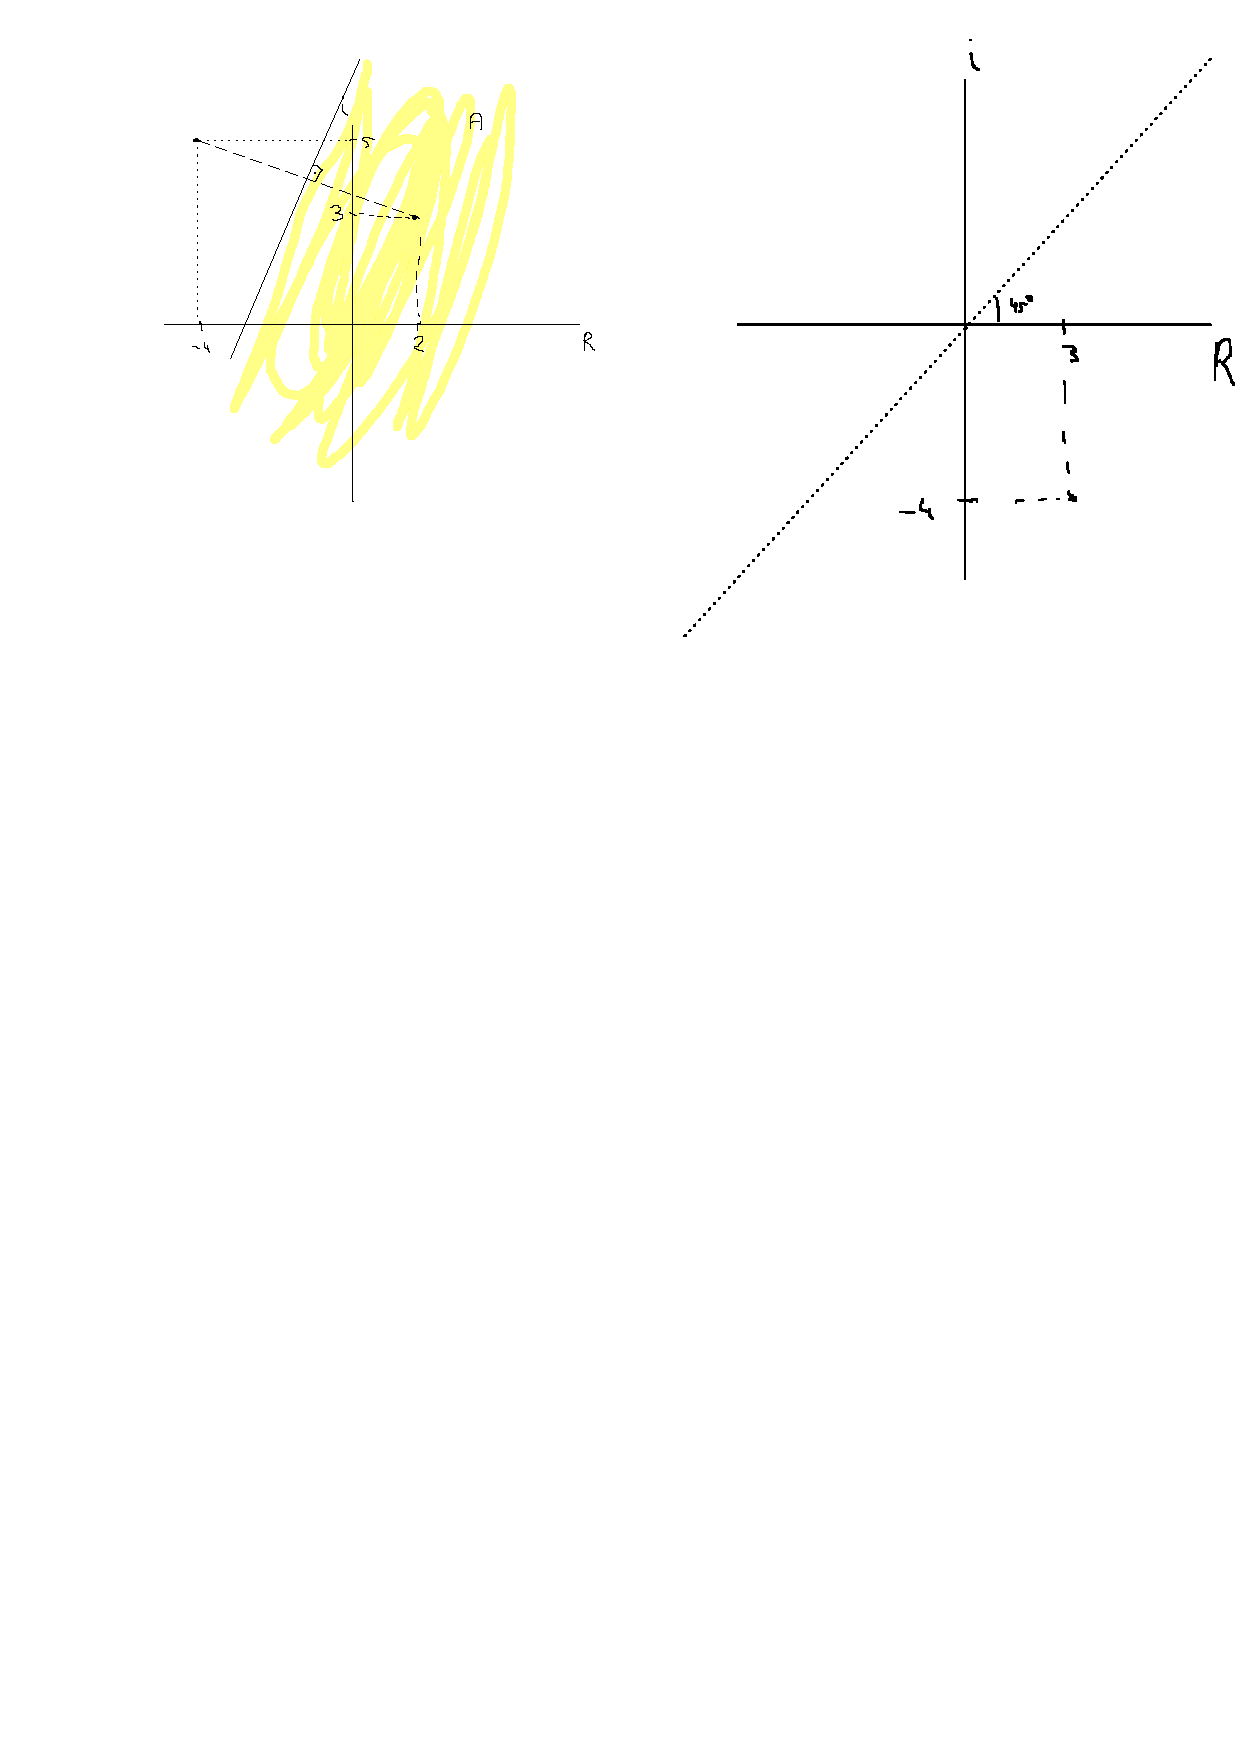
\includegraphics[width=\textwidth]{2025-04-28-Note-13-03.pdf}
    \caption{Visualization for Problem 2}
    \label{fig:problem2}
\end{figure}

\end{document}